\documentclass[11pt,a4paper]{article}
\usepackage[a4paper, margin=0.6in]{geometry}
\usepackage{parskip}
\usepackage{titling}
\usepackage{graphicx}
\graphicspath{{../images/}}
\setlength{\droptitle}{-3em}

\title{COMP4321 Database Schema}
\author{
    Adrian Prawira Susanto\\20369593\\ \texttt{apsusanto@ust.hk} \and
    Kevin Pratama\\20369036\\ \texttt{kpratama@ust.hk} \and
    Randitya Setyawan Mohamad\\20316273\\ \texttt{rsmohamad@ust.hk}}
\date{}

\begin{document}
    \maketitle

    The database consists of several key/value tables that are stored locally on disk.
    The package used for our database manager is BoltDB, a persistent key/value storage for the Go programming language.
    BoltDB's underlying structure for the key/value table is B+ tree, and therefore our tables are implemented as B+ trees.

    As for the schema itself, the tables are partitioned into four main categories:
    \begin{enumerate}
        \item Mappings \\
        These tables contain convenient mapping from one value to another, to allow ease of use during implementation.
        \item Indexes \\
        These tables are one of the most integral part of our search engine.
        The indexes allow for both forward lookup (From DocumentID to the words) and backward lookup (From Word to DocumentID), commonly known as Forward and Inverted index respectively.
        \item Scoring \\
        These tables contain scoring related information and must be updated after a set of pages has been added to the index.
        The scores are precomputed to allow faster retrieval.
        \begin{itemize}
            \item TermWeights stores the term weights ($tf \cdot idf$) of all terms in each page.
            \item AdjList stores the parent IDs of each page, along with the number of links of that parent.
            \item From this AdjList, the PageRank scores are precomputed, which are then stored in the table PageRank.
        \end{itemize}
        \item Page Metadata \\
        The page metadata only has one table, PageInfo, that stores the additional information such as size, last-modified date, and child links.
        The information here will not be directly used by the retrieval engine but will be shown on the result page.

    \end{enumerate}

    \begin{center}
        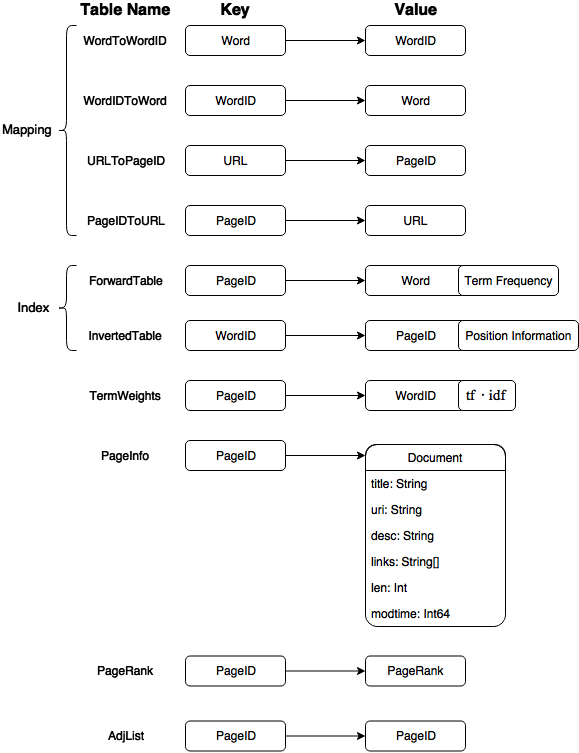
\includegraphics[scale=0.8]{databaseSchema} \\[2\baselineskip]
    \end{center}

\end{document}